\newcommand\multirowline[1]{\begin{tabular}{@{}c@{}}#1\end{tabular}}

\chapter{Evaluation of Porting Costs} \label{sec:eval}

% What I want to say in this section:
%   - I want to take the model of Tanaka and map my timeline on it (maybe merge
%   the model with [1])
%   - I want to talk about the porting tasks
%     - which was most time consuming
%     - which of them were repetitive and added little value
%     - etc
%   - I want to talk about the human and development factors as described in [1]
%   - talk about environment disparity and program factors; and how did this
%   affect the costs
%   - Finally I need to understand the equations for porting costs evaluation
%   and estimation in order to compare the resluts (and maybe talk about the
%   porting productivity index)
%   - I don't know if I should place it here or in implementation chapter but
%   I would like to have a table with portability impedimets,reason for changes,
%   details of changes and need for change in future porting. They do so in
%   Tanaka et al
%
% LucianM proposed to talk about some aspects of the program to be ported as:
%   - size
%   - content
%
% The Tanaka+Hakuta model mapped on our timeline will be presented in a table.
% The indices from Hakuta([1]) will be presented in different section (idk).
%
% [1] "A study of Software Portability Evaluation"

In this section we present the costs associated with the porting process
described in Section~\ref{sec:portingIxos}. We divide our work in tasks
that can be individually evaluated based on the revised model discussed in
Chapter~\ref{sec:revised-porting-model} and describe the methodology of
extracting the porting costs based on the progress tracking we have done during
the project.

Later we discuss the factors that affected our cost evaluation. We focus on
three aspects of these factors: portability impedimets, human experience and
environmental factors. For each of them we analyze a score to understand their
impact in the project and we analyze them with regards to our porting.

\section{Costs of Porting IxOS on ARM Boards}

To evaluate the costs for porting IxOS infrastructure we divided our work based
on the model described in Section~\ref{sec:background}. Using the progress
tracking done during the project, we extracted the time spent on each task. We
use man-hours to evaluate the cost for each task. The results of this process
is shown in Table~\ref{tab:manHoursEvaluation}.

\begin{table*}
\centering
\begin{tabular}{ |l *{5}{|l}| }
\hline
Porting task & Subtasks & \multirowline{Man\\-hours} & \multirowline{Subtotals\\/subtask (\%)} & \multirowline{Subtotals\\/task (\%)} \\
\hline
\multirow{7}{5em}{Advance preparations} & \multirowline{Surveying development \\ environment} & 15   & 4.16 & \multirow{7}{5em}{14.35}\\
                                        \cline{2-4}
                                        & Surveying target OS                                 & 5    & 1.38 &                         \\
                                        \cline{2-4}
                                        & Surveying program for porting                       & 3    & 0.83 &                         \\
                                        \cline{2-4}
                                        & Surveying documentation                             & 5    & 1.38 &                         \\
                                        \cline{2-4}
                                        & \multirowline{Adjusting development \\ environment} & 10   & 2.77 &                         \\
                                        \cline{2-4}
                                        & Adjusting target environment                        & 13.8 & 3.83 &                         \\
                                        \cline{2-4}
                                        & Initial source code modifications                   & 0    & 0    &                         \\
\hline
\multirow{5}{5em}{Building for target environment} & \multirowline{Build system triggering and \\ modification}                          & 67.56 & 18.76 & \multirow{5}{5em}{32.71} \\
                                                   \cline{2-4}
                                                   & \multirowline{Installation on remote \\ environment}                               & 15.26 & 4.23  &                          \\
                                                   \cline{2-4}
                                                   & \multirowline{Reviewing inconsistencies between \\ source and remote environments} & 23.03 & 6.39  &                          \\
                                                   \cline{2-4}
                                                   & \multirowline{Solving problems with external \\ dependencies}                      & 12    & 3.33  &                          \\
\hline
\multirow{2}{5em}{Testing} & Testing in simulated environment & 33.35  & 9.26  & \multirow{2}{5em}{24.53} \\
                           \cline{2-4}
                           & Testing in target environment    & 55     & 15.27 &                          \\
\hline
\multirow{3}{5em}{General duties} & Documentation     & 30 & 8.33  & \multirow{3}{5em}{28.26} \\
                                  \cline{2-4}
                                  & Progress tracking & 12 & 3.33  &                          \\
                                  \cline{2-4}
                                  & Discussions       & 60 & 16.66 &                          \\
\hline
\multirow{1}{5em}{Total} & & 360  & 100 & \multirow{1}{5em}{100}\\
\hline
\end{tabular}
\caption{Man-hours evaluation for porting tasks}
\label{tab:manHoursEvaluation}
\end{table*}

The most time consuming task is \textit{Build system triggering and
modification}. This happened because we spent a lot of time on extracting and
integrating IxOS components as InterfaceManager, HostProxy and IxServer. There
was also much repetitive time spent on triggering the compilation pipeline that
was added in the total of 67 hours.

We spent an approximately 2.5x more time on testing than on solving errors and
inconsistencies. This means that the errors were not difficult to solve, instead
they were difficult to find.~\lm{Could this be one of the golden nuggets to be mentioned in the abstract? Not sure.} This situation is no surprise for us because we had
no reference or documentation that would help us in investigating the errors and
inconsistencies.~\lm{One question here that might help focus this: what exactly should the documentation have comprised that was missing? Was it a detailed architecture of IxOS? Implementation specifics (e.g. the ethtool thing on IxVM card)? Something else altogether? I'm also asking this because I'm actively seeking to improve the IxOS technical documentation, among others.}
\lp{I think that a more comprehensive diagram of the architecture details
specific to our porting whould have been very helpful, furthermore
implementaiton details for chassis and card would have also helped. I think that
any kind of documentation would have helped in this situation. \textit{However},
looking back at the project and at this one year that passed and in which I
gathered some experience with software engineering by working on other large
systems, I can say that documentation is not the only factor that can make the
project easier or harder. The time spent on the project is much more important
than documentation. I think it's clear why: you take time to get familiar with
the project and understand the components of the system by solving errors,
getting to know implementation details that might not be present in documentaion
and by communicating with other people that are involved in the project}

There was no time allocated on making initial source code modifications because
the system was unfamiliar and hard to understand from the start. Finally, we
spent more time on \textit{General Duties} than on \textit{Testing}. This shows
that there was a substantial effort put in trying to make use of discussions
to clarify the system. In the end we suceeded in porting the system, meaning
that the discussions we had helped us to clarify the various parts of the system
that were not understood in the beginning.

\section{Methodology of extracting costs of porting}

To extract the costs of porting we used the progress tracking created during the
12 weeks of porting. Each week we allocated one hour to discuss the current
status of the project and the items we plan to do in the following week. A
sample of our tracking looks as following:

\begin{verbatim}
# 02.08 - 06.08

Status
  * IM is booting, having config issues
  * created RPi setup
  * deployed RPi + vChassis + IxExplorer setup
    * port is visible from IxE but we have issues with link state
      * maybe there is a problem with published stats
  * attempted connections from vChassis to vCard
  * ran into configuration issues
  * need to trick the vChassis into beliving that we're on x64

Planning
  * fix port down/hwfault report from IM
    * trick the chassis into beliving we're legit IxVM
    * make HostProxy - chassis connection
\end{verbatim}

During a week we allocated 30 hours for porting. 5 hours were allocated to daily
meetings were we discussed the plan for the respective day and 1 hour a week was
allocated to progress tracking, resulting in 24 hours of work for solving
technical problems related to porting. To convert the weekly tasks recorded in
the tracking in the effective man-hours presented
in Table~\ref{tab:manHoursEvaluation}, we matched each porting task on the
progress tracking task. At first, the total amount of 24 hours is divided
equally between the porting tasks, following adjustments based on factors as
difficulty and frequency.

Let us take the above example to extract the porting tasks from the progress
tracking tasks.

\begin{itemize}
\item IM is booting, having config issues :
    \begin{itemize}
    \item Build system trigging and modifications
    \item Installation on remote environment
    \item Reviewing inconsistencies between source and remote environments
    \item Testing in simulated environment
    \end{itemize}

\item created RPi setup
    \begin{itemize}
    \item Adjusting target environment
    \end{itemize}

\item deployed RPi + vChassis + IxExplorer setup, port is visible from IxE but
we have issues with link state, maybe there is a problem with published stats
    \begin{itemize}
    \item Adjusting target environment
    \item Reviewing inconsistencies between source and remote environments
    \end{itemize}

\item attempted connections from vChassis to vCard
    \begin{itemize}
    \item Testing in target environment
    \end{itemize}

\item ran into configuration issues
    \begin{itemize}
    \item Testing in target environment
    \item Reviewing inconsistencies between source and remote environments
    \end{itemize}

\item need to trick the vChassis into beliving that we're on x64
    \begin{itemize}
    \item Reviewing inconsistencies between source and remote environments
    \end{itemize}
\end{itemize}

We have six different porting tasks that we must allocate time to. Each task has
4.16 hours initially. However, \textit{Build system triggering and modification}
did not take this long, neither did \textit{Installatino on remote environment}.
These are task that will have less time allocated than the initial 4.16 hours.
We will have 2 hours for Build system triggering and modifications and 1 hour
for Installation on remote environment. The remaining 4.32 hours will be
allocated evenly to the remaining four tasks. Finally we have the following
results for the week:
\begin{itemize}
    \item Advance preparations
        \begin{itemize}
            \item Adjusting target environment: \textbf{5.24 hours}
        \end{itemize}
    \item Building for target environment
        \begin{itemize}
            \item Build system triggering and modification: \textbf{2 hours}
            \item Installation on remote environment: \textbf{1 hour}
            \item Reviewing inconsistencies between source and remote
            environments: \textbf{5.24 hours}
        \end{itemize}
    \item Testing
        \begin{itemize}
            \item Testing in simulated environment: \textbf{5.24 hours}
            \item Testing in target environment: \textbf{5.24 hours}
        \end{itemize}
    \item General duties
        \begin{itemize}
            \item Progress tracking: \textbf{1 hour}
            \item Discussions: \textbf{5 hours}
        \end{itemize}
\end{itemize}

After this algorithm is applied on each week we get the results in~Table~\ref{tab:manHoursEvaluation}.

\section{Factors of porting costs}

While the costs of porting, in our case man-hours, are determined directly by
program size and content, other factors and impediments as human experience and
environment disparities must be taken into consideration.

To determine the impact some of these factors had on our porting process, we
use the indices described in Hakuta and Ohminami~\cite{hakuta} that give
a quantitative influence of porting factors and impediments.

\subsection{Portability Impediment Index}

The first index that we compute is the portability impediment index. In our
case $eta$ has a value of 2, meaning that "the non-portable parts of the program
are not localized, but the correspondence of program codes to their functions is
clarified". For simplicity we will assume that $\omega_i$ is 0 if the impediment
was insignificant, 0.5 if the impediment had a normal difficulty and 1 if the
impediment was hard to solve. In our porting we discovered the following
portability impediments:
\begin{itemize}
    \item Difference in compiler specification (S8)
    \item Scope of library support (S9)
    \item Implementation-dependent libraries (S10)
    \item Difference in operating system interface (S12)
\end{itemize}

It can be noted that we added an additional impediment nonexistent in Hakuta and
Ohminami's list~\cite{hakuta}, namely S12, which can be placed in the "OS disparity"
category. This impediment is reflected in the usage of dmidecode(8) on Raspberry
Pi Linux versus on x86 Linux. On Raspberry Pi we were not allowed to access
/dev/kmem which was needed by dmidecode(8), which in turn was needed by
InterfaceManager.

Given these impediments the portability impediment index has the following
value: $\alpha_p = 2 * (0.5 * S8 + 1 * S9 + 1 * S10 + 0.5 * S12) = 6$.  There
were no differences between processor architecture (S1$\sim$S5), little difference
between source and target OSes (S6, S7, S12) and a major difference in language
processor (S8$\sim$S11). The portability difficulty is thus reflected in
Figure~\ref{fig:pii}.

\begin{figure}
    \begin{center}
    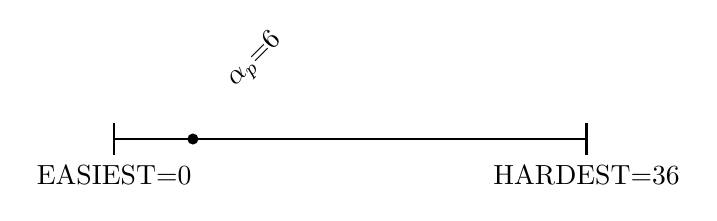
\begin{tikzpicture}[
        dot/.style = {circle, fill=black,inner sep=0pt, minimum size=4pt},
        every label/.append style = {inner sep=0pt, rotate around={45:(-0.5,1.5)}},
            thick      
    ]
        \draw (0,0.2) -- + (0,-0.4) node[below] {EASIEST=0};
        \draw (6,0.2) -- + (0,-0.4) node[below] {HARDEST=36};
        \draw[thick] (0,0) -- node[below=2mm] {} + (6,0);
        \node[dot,label={$\alpha_p$=6}] at (1,0) {};
    \end{tikzpicture}
    \end{center}

    \caption{Portability Impediment Index}
    \label{fig:pii}
\end{figure}


\subsection{Human Factors Index}

Software programs are byproducts of human activities than incorporate our
problem-solving capabilities, cognitive aspects and social
interaction~\cite{capretz}, therefore it is vital to understand what role did the
human factors play in our porting so that we can assess the quality of the
porting process. 

In our case $\alpha_h = H1 + H2 + H3 + H4 + H5 = 2 + (-1) + 2 + 1 + 2 = 6$.
This score is very close the worst possible score as seen in
Figure~\ref{fig:hfi}.

\begin{figure}
    \begin{center}
    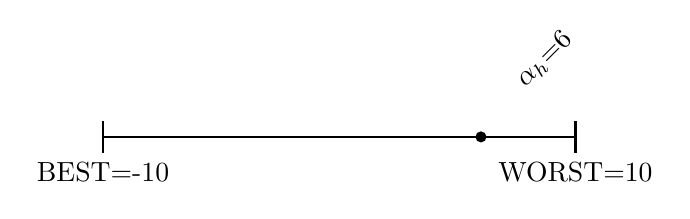
\begin{tikzpicture}[
        dot/.style = {circle, fill=black,inner sep=0pt, minimum size=4pt},
        every label/.append style = {inner sep=0pt, rotate around={45:(-0.5,1.5)}},
            thick      
    ]
        \draw (0,0.2) -- + (0,-0.4) node[below] {BEST=-10};
        \draw (6,0.2) -- + (0,-0.4) node[below] {WORST=10};
        \draw[thick] (0,0) -- node[below=2mm] {} + (6,0);
        \node[dot,label={$\alpha_h$=6}] at (4.8,0) {};
    \end{tikzpicture}
    \end{center}

    \caption{Human Factors Index}
    \label{fig:hfi}
\end{figure}

Indeed, the human factor played a major role in our porting process, let
us analyze each factor and see what went wrong.

\paragraph{Knowledge about the program to be ported functions and structures
(H1)}
As this was the first interaction with the program to be ported it was
hard to familiarize with its functions and structures, therefore we had no
experience whatsoever with the use cases of the program. This resulted in the
inability to easily solve the porting problems that appeared in our way.

\paragraph{Knowledge about the hardware and OS of the target system (H2)}
Hardware disparities were not a big concern in our porting as we used a portable
operating system and programming language that abstracted out hardware problems.
Therefore the focus was on the target operating system. Our porting moved the
program from an older version of Linux to a newer one. This helped us as we
did not have to learn the peculiarities of another operating system so that we
could finish our porting. However there were some problems that we faced
regarding the target operating system that we solved relatively straight
forward.

\paragraph{Knowledge and experience in the area of software porting (H3)}
As the experience of software porting was lacking there were many situations
and problems that could have been solved better, for example: doing better
tracking of the porting process, putting more effort in technical discussions
in order to better understand the problems, etc.

\paragraph{Knowledge of and experience with the language and program to be ported
in use(H4)}
The experience with the programming language (C++) helped us to grow the
productivity of the porting process as we did not have to care about low-level
impediments as endianness or data alignment. However we did have problems with
the language specification between different compilation toolchains that costed
us a whole week to solve. Furthermore, the experience with use cases of the program
to be ported was lacking. 

\paragraph{Knowledge about the functions and usage of tools used in the development
and testing environment (H5)}
While working in the development and testing environments we used a considerable
number of technologies, some of them being either new or not trivial to work
with. Here is a short list of these technologies: QEMU networking, SCons build
system, Perforce versioning system and internal tools as packaging system. This
meant that we had to allocate additional time to ramp-up with each of this tools
after continuing with our goal.

\subsection{Environmental Factors Index}

The tools used in the development environment and the testing mechanisms used in
the testing environment also add their bit in the porting costs.

In the development environment we had no documentation describing the compiling
and linking procedures and no documentation regarding the environment dependent
components that we need to modify in order to move the code to a new
environment. We modified the code and the build system by trial and error. This
reduces the score for E1 as this strategy might not always work or it could take
an unsatisfactory amount of time for large and complicated systems. However
we managed to understand the peculiarities of the development environment and
get the first builds available for testing in two or three weeks, which is less
than 25\% of our porting time.

In the testing environment we had test programs and tools available such as
emulators and debuggers, furthermore the file transfer and conversion tools
were available from the start of the project. This facilitated the testing of
our program to be ported by allowing us to focus on the porting inconsistencies
rather than on testing infrastructure. Things were not perfect however, we did
have problems with the testing infrastructure that we solved in a short period
of time.

The environmental factors index has the following value in our case: $\alpha_e =
E1 + E2 + E3 = 0 + NA + -1 = -1$. We are in the satisfactory half of the index,
meaning that even if we had some difficulties setting and understanding the
development and testing environment, we managed to work with them in order to
achieve our goals. The score is also described in Figure~\ref{fig:efi}.

\begin{figure}
    \begin{center}
    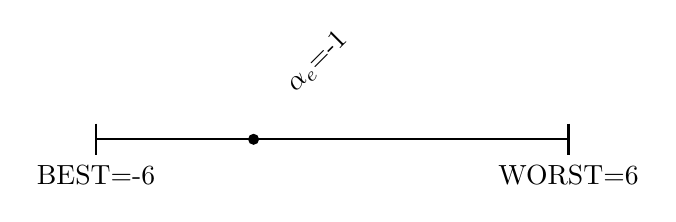
\begin{tikzpicture}[
        dot/.style = {circle, fill=black,inner sep=0pt, minimum size=4pt},
        every label/.append style = {inner sep=0pt, rotate around={45:(-0.5,1.5)}},
            thick      
    ]
        \draw (0,0.2) -- + (0,-0.4) node[below] {BEST=-6};
        \draw (6,0.2) -- + (0,-0.4) node[below] {WORST=6};
        \draw[thick] (0,0) -- node[below=2mm] {} + (6,0);
        \node[dot,label={$\alpha_e$=-1}] at (2,0) {};
    \end{tikzpicture}
    \end{center}

    \caption{Environmental Factors Index}
    \label{fig:efi}
\end{figure}

Now that we evaluated the costs and discovered their correlation with the porting
factors we will conduct a discussion on the results of our evaluation.
